\author[Christopher Schwan]{}
\institute{Universit\`a di Milano}

\subsection{Electroweak corrections}

\begin{frame}{NLO EW corrections for PDF fits}
\fontsize{9}{11}\selectfont
\begin{columns}[onlytextwidth]
\begin{column}{0.45\textwidth}

\begin{block}{Ingredients?}
\begin{itemize}
\item[\ding{51}] At least QED corrections in DGLAP
\item[\ding{51}] Non-zero photon (lepton, \ldots) PDF
\item[(\ding{55})] NLO EW (+ NLO QCD+EW) corrections for all PDF processes
\end{itemize}
\end{block}

\vspace*{0.2cm}

\begin{block}{Motivation?}
\begin{itemize}
\item Below \SI{1}{\percent} NLO EW will matter!
\item Cuts can be relaxed: DY large-mass region, large Z $p_\mathrm{T}$, \ldots
\item User demand
\end{itemize}
\end{block}
\end{column}
\begin{column}{0.45\textwidth}
\begin{block}{Problems to be solved}
\begin{itemize}
\item[\ding{51}] Need corrections in the form of \alert{interpolation grids}: PineAPPL, interfacing with Madgraph5\_aMC@NLO, see\\
\beamercite{S.\ Carrazza, E.R.\ Nocera, C.S., M.\ Zaro}{https://inspirehep.net/literature/1814432}
\item[\ding{51}] Careful selection of data: no subtraction of FSR, no photon-initiated subtraction, proper observable definition\\
see my \href{https://indico.cern.ch/event/941711/contributions/4020188/}{LHCEWWG 2020 talk}
\item[\ding{55}] Write/verify runcards and run them (WIP)
\item[\ding{55}] Implement changed data (WIP)
\item[$\rightarrow$] Run fit
\end{itemize}
\end{block}
\end{column}
\end{columns}
\end{frame}

\begin{frame}[t]{Example: Drell--Yan @ 14 TeV}
\fontsize{9}{11}\selectfont
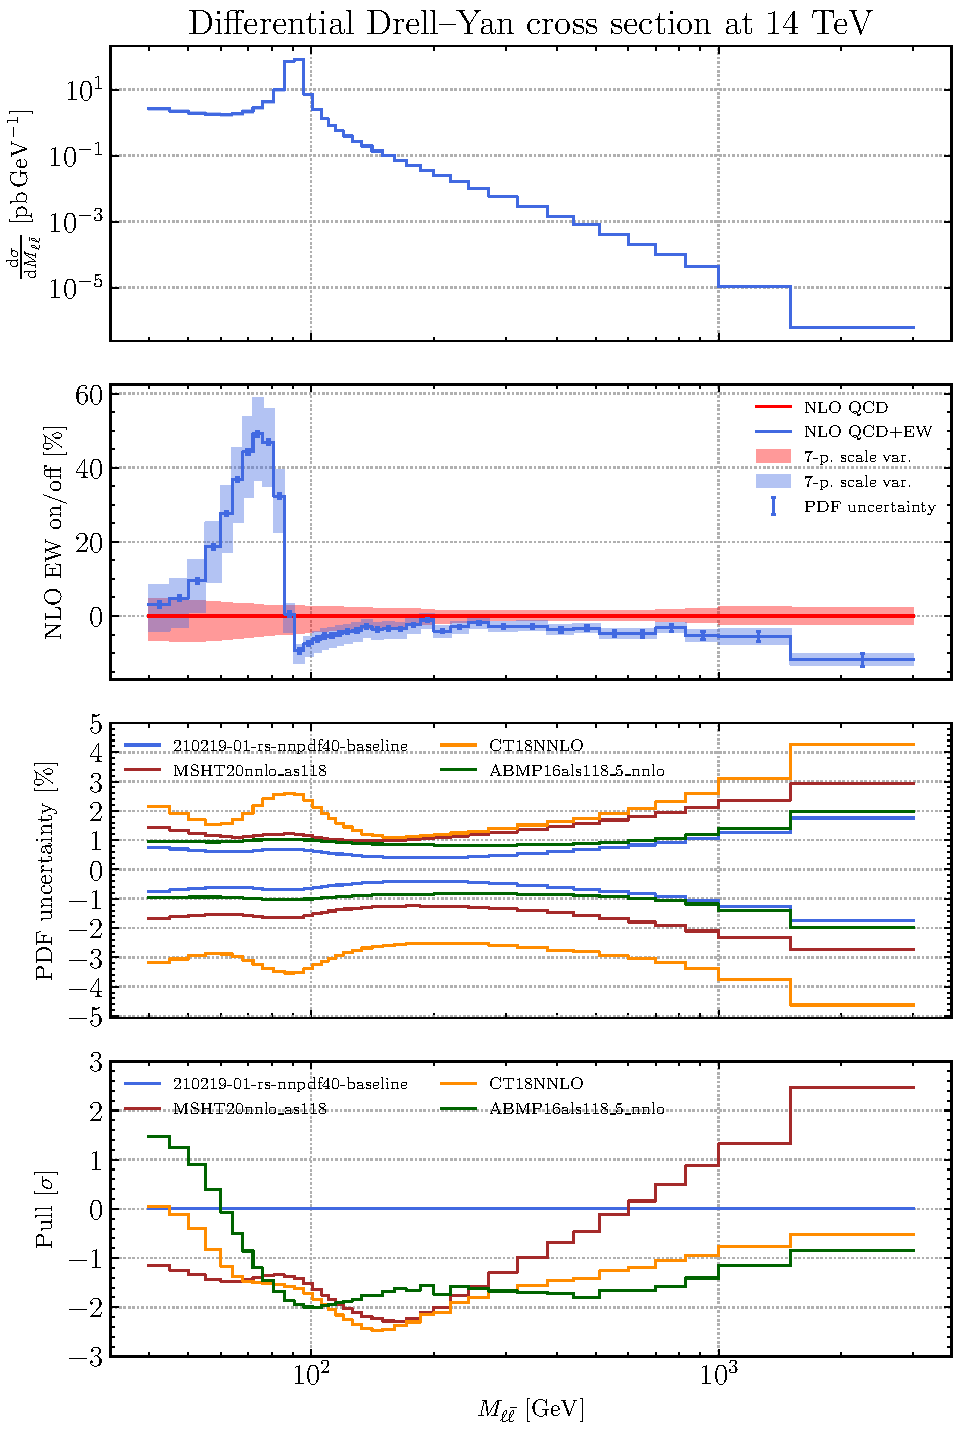
\includegraphics[trim=0 350 0 0,clip,width=0.5\textwidth]{ew_corrections/figures/NNPDF40_DY_Z-global}%
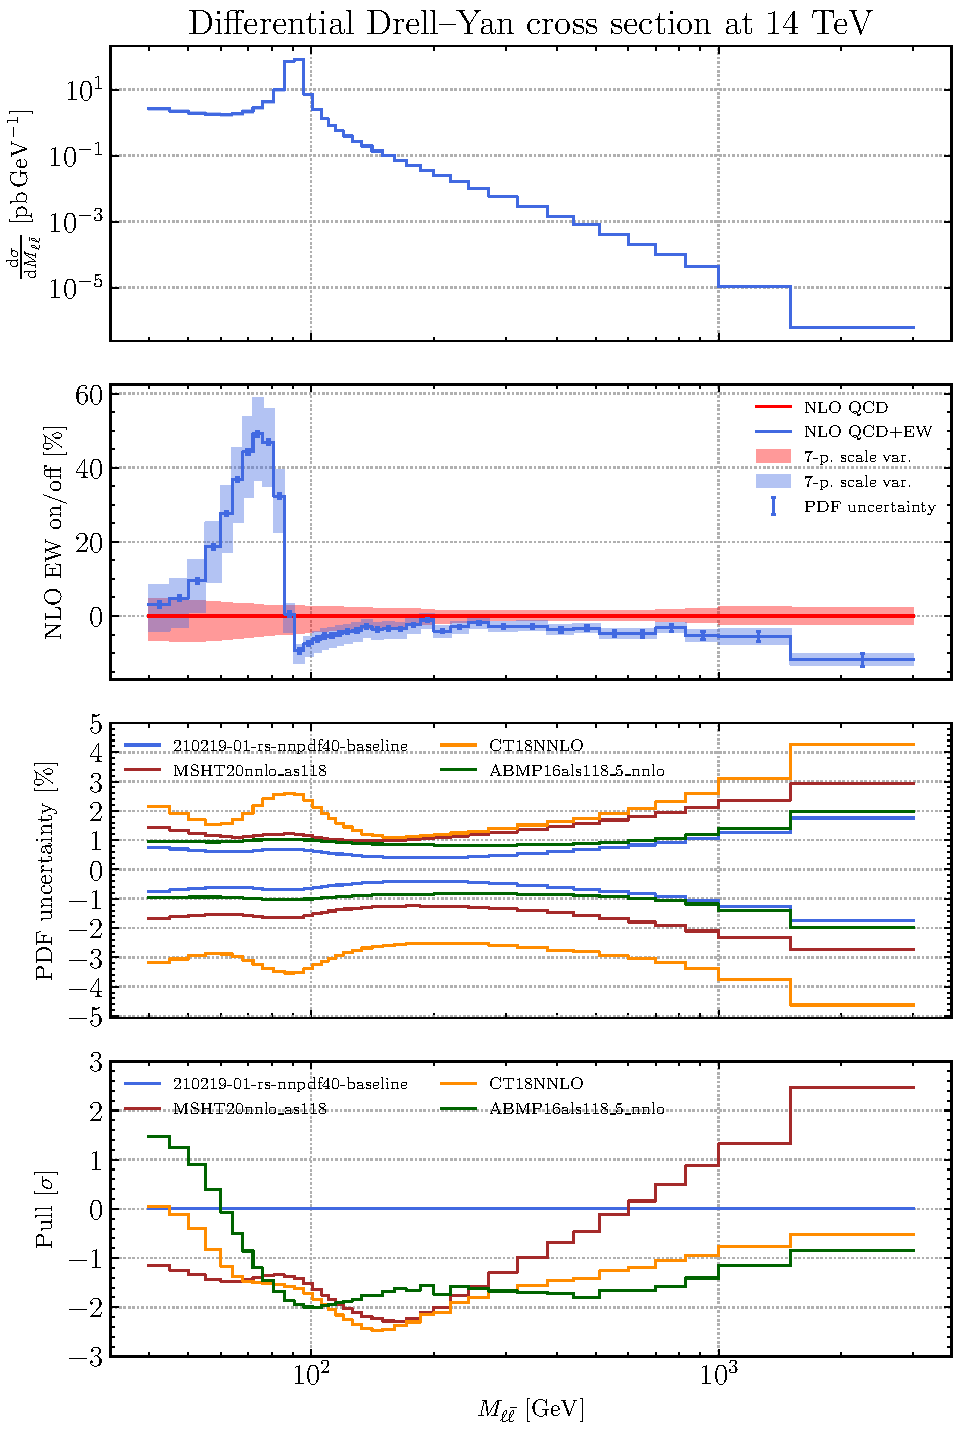
\includegraphics[trim=0 0 0 330,clip,width=0.5\textwidth]{ew_corrections/figures/NNPDF40_DY_Z-global}
\begin{columns}[T,onlytextwidth]
\begin{column}{0.5\textwidth}
\begin{itemize}
\item binning from CMS DY @ \SI{13}{\tera\electronvolt}: \href{https://arxiv.org/abs/1812.10529}{arXiv:1812.10529}
\item FSR distort the Z peak, weak corrections in the large-mass region
\end{itemize}
\end{column}
\begin{column}{0.5\textwidth}
\begin{itemize}
\item PDF uncertainties for NNPDF4.0, CT18NNLO, MSHT20, and ABMP16
\end{itemize}
\end{column}
\end{columns}
\end{frame}
